In this chapter, we introduce the version of PMCLP where every 
facility has an axis-parallel ellipse as its coverage area. We refer to this problem as \sigla{MCE}{Maximum Covering by Ellipses}. We also present an algorithm for it which is an adaptation of the one developed for MCD in \autoref{chapter:pmclp}.

\section{Definition}

Axis-parallel ellipses are defined as the set of points that satisfy \autoref{equation:pellipse}. All it takes to describe one is a pair of positive real numbers $(a,b) \in \R_{>0}^2$, with $a>b$, also called its shape parameters, and a center $q \in \R^2$.

An instance of MCE is given by a set of $n$ demand points $\Pp = \{p_1, \dots, p_n\}$, with $p_j\in\R^2$; 
a set of weights $\Ww:=\{w_1, \dots, w_n\}$, with $w_j\in\R_{\ge0}$ being the weight of point $p_j$;
and a set of $m$ axis-parallel ellipses given by their shape parameters $\Rr:=\{(a_1, b_1), \dots, (a_m, b_m)\}$, with $(a_j, b_j)\in\R_{>0}^2$ and $a_j>b_j$.
Additionally, to make the text more clear, we define a set $\E = \{E_1, \dots, E_m\}$, with $E_j : \R^2 \mapsto \R^2$ being a function that takes the center where the $j$-th ellipse is located as input, and returns its coverage region as defined by \autoref{equation:cover_pellipse}.

A solution for MCE is given by $Q:=(q_1, \dots, q_m)\in\R^{2m}$, with $q_j$ being the center of $j$-th ellipse. Let $w : 2^\Pp \mapsto \R_{\ge0}$ as defined by \autoref{eq:subset_w}, then an optimal solution of MCE is given by the optimization problem

\begin{equation*}
\max_q w\left(\bigcup_{j=1}^m \Pp \cap E_j(q_j)\right).
\end{equation*}

In the next sections, we first study the specific case of MCE with only one facility and discuss that the results of \autoref{chapter:pmclp} still apply when ellipses are used instead of disks. After that, we use the approach mentioned in \autoref{chapter:pmclp} of constructing a CLS for each facility and propose an algorithm for MCE.

\section{Related work}
The maximal planar covering using axis-parallel ellipses was first introduced in \citeonline{canbolat} which proposed a mixed integer non-linear programming method for the problem. This first approach showed to be not that efficient as it could not find an optimal solution for some instances within a timeout defined by them. To obtain solutions, not necessarily optimal ones, for the instances which the exact method showed inefficiency, a heuristic technique called Simulated Annealing was used to develop another method. Comparisons were made, which showed that the second approach was able to obtain good solutions, compared to the optimal ones found for some of the instances, within a good run-time.

The second work found in the literature was \citeonline{andreta}, which developed a method that breaks the problem into smaller ones fixing the set of points an ellipse is going to cover. For each set of points fixed as the points an ellipse is going to cover, a small optimization problem is solved to find out if there is a location where the ellipse can be placed, so to cover the set of fixed points. To enumerate the possible solutions and then find an optimal one, the method defined a data structure that stores every set of points an ellipse can cover. This method showed better results and was able to find optimal solutions for the instances that the first method could not get as well as for new created instances.

\section{One Ellipse Version}

The case with only one ellipse is considered first because it will be adapted to become the basis of the algorithm for more than one ellipse. We refer to this version as \sigla{MCE1}{Maximum Cover by One Ellipse}. 

An instance of MCE1 has $m=1$, and we set $(a, b):=(a_1, b_1)$, and $\E := \{E\}$. Therefore, an instance of MCE1 is described by the tuple $(\Pp; \Ww; (a, b))$. A solution of MCE1 is then given by a point $q\in\R^2$, and an optimal solution is given by the optimization problem

\begin{equation*}
\max_q w(\Pp \cap E(q)).
\end{equation*}
An adaptation of \autoref{algoritmo:mcd_1} is obtained by just replacing the function that finds the intersection points between two disks by a function that finds the intersection points between two ellipses $\partial E_i$ and $\partial E_j$.
It can be seen in \autoref{fig:3ellipses_intersect} that the intersection points and their correspondents $\Gamma_-(i,j)$ and $\Gamma_+(i,j)$ functions behave the same way as in the disks case.
The intersection of two ellipses as well as determining $\Gamma_-(i,j)$ and $\Gamma_+(i,j)$ are described in the next section.

\begin{figure}[H]
	\centering
	\caption{Three ellipses and their intersection points}
	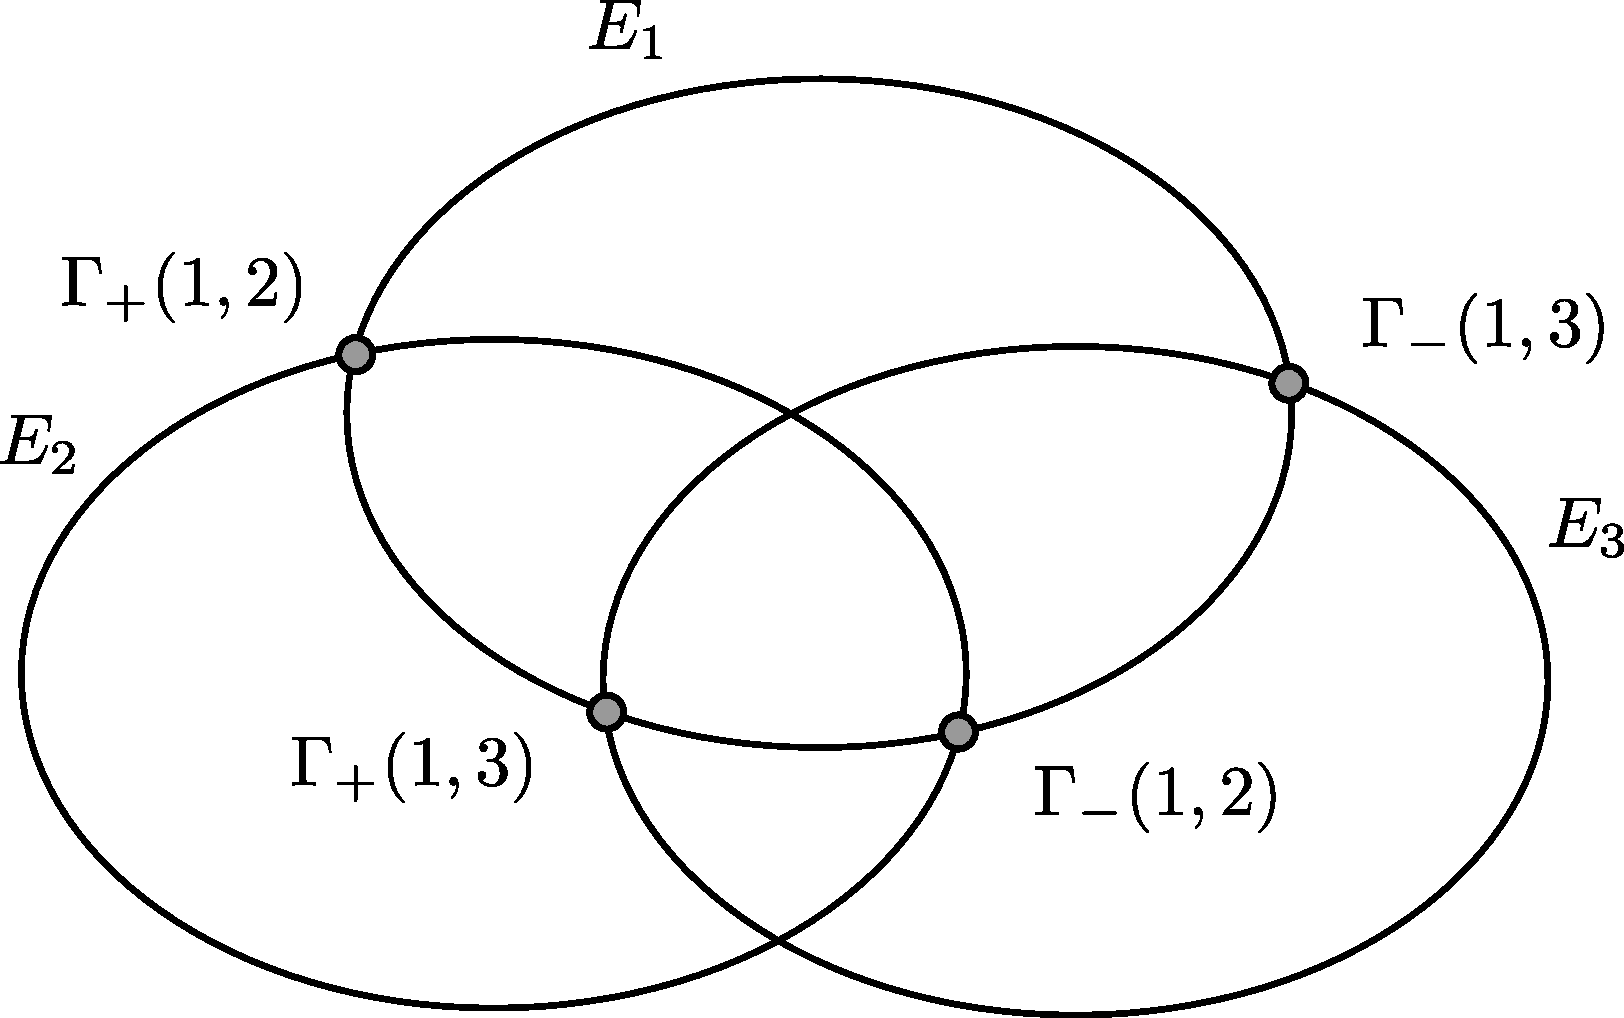
\includegraphics[scale=.34]{tex/figures/3ellipses_intersect.pdf}
	\fautor
	\label{fig:3ellipses_intersect}
\end{figure}

\section{Determining $\Gamma_+(i,j)$ and $\Gamma_-(i,j)$}\label{section:ellipses_intersection}

Let $E_1(q_1)$, and $E_2(q_2)$ be two coverage region of ellipses centered at $q_1, q_2\in\R^2$ respectively, with shape parameters $(a, b)\in\R^2_{>0}$. After changing the coordinates to make the center of the first ellipse be at the origin, the intersection points between the two ellipses are defined by

\begin{align}
\frac{x^2}{a^2} + \frac{y^2}{b^2} = 1 && (E_1) \label{eq:ell_inter_1}\\
\frac{(x-h)^2}{a^2} + \frac{(y-k)^2}{b^2} = 1 && (E_2), \nonumber
\end{align}
where $(h,k)\in\R^2$ is the center of the second ellipse after the coordinates were translated by $-q_1$. As both equations are equal to $1$, we have
\begin{align}
    b^2x^2 + a^2y^2 &= b^2(x-h)^2 + a^2(y-k)^2 \nonumber\\
    x &= y\frac{-2ka^2}{2hb^2} + \frac{b^2h^2 + a^2k^2}{2hb^2} \nonumber\\
    x &= y\alpha + \beta.\label{eq:ell_inter_2}
\end{align}
Replacing \autoref{eq:ell_inter_2} into \autoref{eq:ell_inter_1}, we get
\begin{align}\label{eq:ell_inter_3}
y^2(b^2\alpha^2 + a^2) + y(2\beta\alpha b^2) + b^2\beta^2 -a^2b^2 = 0,
\end{align}
which is a second degree polynomial. Then, $\partial E_1(q_1) \cap \partial E_2(q_2) \neq \{\}$ if, and only if the roots of \autoref{eq:ell_inter_3} are real. The intersection points itself can be obtained by solving the polynomial for $y$ and plugging its value back into the $x=y\alpha + \beta$ equation.

Suppose that $\partial E_1(q_1) \cap \partial E_2(q_2) = \{p_1, p_2\}$, with $p_1 \neq p_2$. To determine $\Gamma_+(1,2)$ and $\Gamma_-(1,2)$, we need to first determine the intersection angles corresponding to $p_1$ and $p_2$ on $E_1(q_1)$. 

Let $\gamma_1$ and $\gamma_2$ be two curves defined as \autoref{eq:parametric_ellipse} for $E_1(q_1)$ and $E_2(q_2)$ respectively. 
The intersection angle of $p_i$ in $E_j(q_j)$ is defined as $t_i^{(j)} \in [0, 2\pi)$, such that $\gamma_j(t_i^{(j)}) = p_i$, for $i, j \in \{1, 2\}$. Obtaining $t_i^{(j)}$ can be done analytically solving the equation

\begin{equation*}
	\dfrac{a}{b}\dfrac{p_{iy}-q_{jy}}{p_{ix}-q_{jx}} = \tan{(t_i^{(j)})}.
\end{equation*}

Let $\gamma_1'$ and $\gamma_2'$ be the derivatives of $\gamma_1$ and $\gamma_2$ respectively as defined by \autoref{eq:der_parametric_ellipse}. Then, considering the tangent vectors $\gamma_1'(t_i^{(1)})$ and $-\gamma_2'(t_i^{(2)})$, $i\in \{1, 2\}$, as shown in \autoref{fig:ellipse_gamma}, we can define a function $\phi_{1,2}\colon \{p_1, p_2\} \to \{\Gamma_+(1,2), \Gamma_-(1,2)\}$ that takes an intersection point and returns its corresponding closing/opening intersection angle as

\begin{equation*}
\phi_{1,2}(p_i) = \begin{cases}
\Gamma_+(1,2) & angle(\gamma_1'(t_i^{(1)}), -\gamma_2(t_i^{(2)})) > \pi\\
\Gamma_-(1,2) & angle(\gamma_1'(t_i^{(1)}), -\gamma_2(t_i^{(2)})) < \pi.
\end{cases}
\end{equation*}
Lastly, the case where that angle is equal to $\pi$ happens only when both ellipses intersect at only one point. This case has to be treated separately as, by \autoref{def:inter_arc}, we need to have two equal intersection points: one as $\Gamma_+(1,2)$ and the other as $\Gamma_-(1,2)$.

\begin{figure}
	\centering
	
	\caption{Determining $\Gamma_+(1,2)$ and $\Gamma_-(1,2)$.}
	%\usetikzlibrary{matrix}



\tikzset{every picture/.style={line width=0.75pt}} %set default line width to 0.75pt        

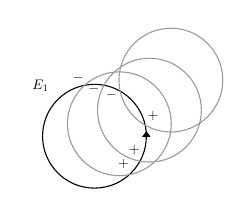
\begin{tikzpicture}[x=0.75pt,y=0.75pt,yscale=-1,xscale=1]
%uncomment if require: \path (0,95); %set diagram left start at 0, and has height of 95

%Shape: Circle [id:dp37777408295388804] 
\draw   (21,59.5) .. controls (21,45.69) and (32.19,34.5) .. (46,34.5) .. controls (59.81,34.5) and (71,45.69) .. (71,59.5) .. controls (71,73.31) and (59.81,84.5) .. (46,84.5) .. controls (32.19,84.5) and (21,73.31) .. (21,59.5) -- cycle ;
%Shape: Circle [id:dp4562198988843913] 
\draw  [color={rgb, 255:red, 155; green, 155; blue, 155 }  ,draw opacity=1 ] (47.5,46.94) .. controls (47.5,33.14) and (58.69,21.94) .. (72.5,21.94) .. controls (86.31,21.94) and (97.5,33.14) .. (97.5,46.94) .. controls (97.5,60.75) and (86.31,71.94) .. (72.5,71.94) .. controls (58.69,71.94) and (47.5,60.75) .. (47.5,46.94) -- cycle ;
%Shape: Circle [id:dp8913971633985722] 
\draw  [color={rgb, 255:red, 155; green, 155; blue, 155 }  ,draw opacity=1 ] (33,53.5) .. controls (33,39.69) and (44.19,28.5) .. (58,28.5) .. controls (71.81,28.5) and (83,39.69) .. (83,53.5) .. controls (83,67.31) and (71.81,78.5) .. (58,78.5) .. controls (44.19,78.5) and (33,67.31) .. (33,53.5) -- cycle ;
%Shape: Circle [id:dp05970043129919356] 
\draw  [color={rgb, 255:red, 155; green, 155; blue, 155 }  ,draw opacity=1 ] (57.81,32.47) .. controls (57.81,18.66) and (69,7.47) .. (82.81,7.47) .. controls (96.62,7.47) and (107.81,18.66) .. (107.81,32.47) .. controls (107.81,46.27) and (96.62,57.47) .. (82.81,57.47) .. controls (69,57.47) and (57.81,46.27) .. (57.81,32.47) -- cycle ;
%Straight Lines [id:da04725899028195979] 
%\draw[densely dotted]  (21,59.5) -- (71,59.5) ;


%Flowchart: Extract [id:dp5267407418119328] 
\draw  [fill={rgb, 255:red, 0; green, 0; blue, 0 }  ,fill opacity=1 ] (71,57.45) -- (72.52,59.55) -- (69.48,59.55) -- cycle ;

\draw (60,73) node [scale=0.5]  {$+$};
% Text Node
\draw (65.22,66) node [scale=0.5]  {$+$};
% Text Node
\draw (74.22,50) node [scale=0.5]  {$+$};
% Text Node
\draw (54.22,39.56) node [scale=0.5]  {$-$};
% Text Node
\draw (45.62,36.96) node [scale=0.5]  {$-$};
% Text Node
\draw (38.02,31.56) node [scale=0.5]  {$-$};


% Text Node
\draw (20,35) node [scale=0.5]  {$E_{1}$};
\end{tikzpicture}

\begin{tikzpicture}

\matrix [matrix of nodes,row sep=,row sep=0mm,
column 1/.style={nodes={rectangle,draw,minimum width=1.5em, minimum height=0.5em}},
column 2/.style={nodes={rectangle,draw,minimum width=1.5em, minimum height=0.5em}},
column 3/.style={nodes={rectangle,draw,minimum width=1.5em, minimum height=0.5em}},
column 4/.style={nodes={rectangle,draw,minimum width=1.5em, minimum height=0.5em}},
column 5/.style={nodes={rectangle,draw,minimum width=1.5em, minimum height=0.5em}},
column 6/.style={nodes={rectangle,draw,minimum width=1.5em, minimum height=0.5em}},
column 7/.style={nodes={rectangle,draw,minimum width=1.5em, color=gray, minimum height=0.5em}},
column 8/.style={nodes={rectangle,draw,minimum width=1.5em, color=gray, minimum height=0.5em}},
column 9/.style={nodes={rectangle,draw,minimum width=1.5em, color=gray, minimum height=0.5em}},
column 10/.style={nodes={rectangle,draw,minimum width=1.5em, color=gray, minimum height=0.5em}},
column 11/.style={nodes={rectangle,draw,minimum width=1.5em, color=gray, minimum height=0.5em}},
column 12/.style={nodes={rectangle,draw,minimum width=1.5em, color=gray, minimum height=0.5em}}
] (O)
{
$+$ & $-$ & $-$ & $-$ & $+$ & $+$ & $+$ & $-$ & $-$ & $-$ & $+$ & $+$\\
%$+$ & $-$ & $-$ & $-$ & $+$ & $+$\\
};

\node at (-4,-0.5) {$0$};
\node at (0,-0.5) {$2\pi$};
\end{tikzpicture}
	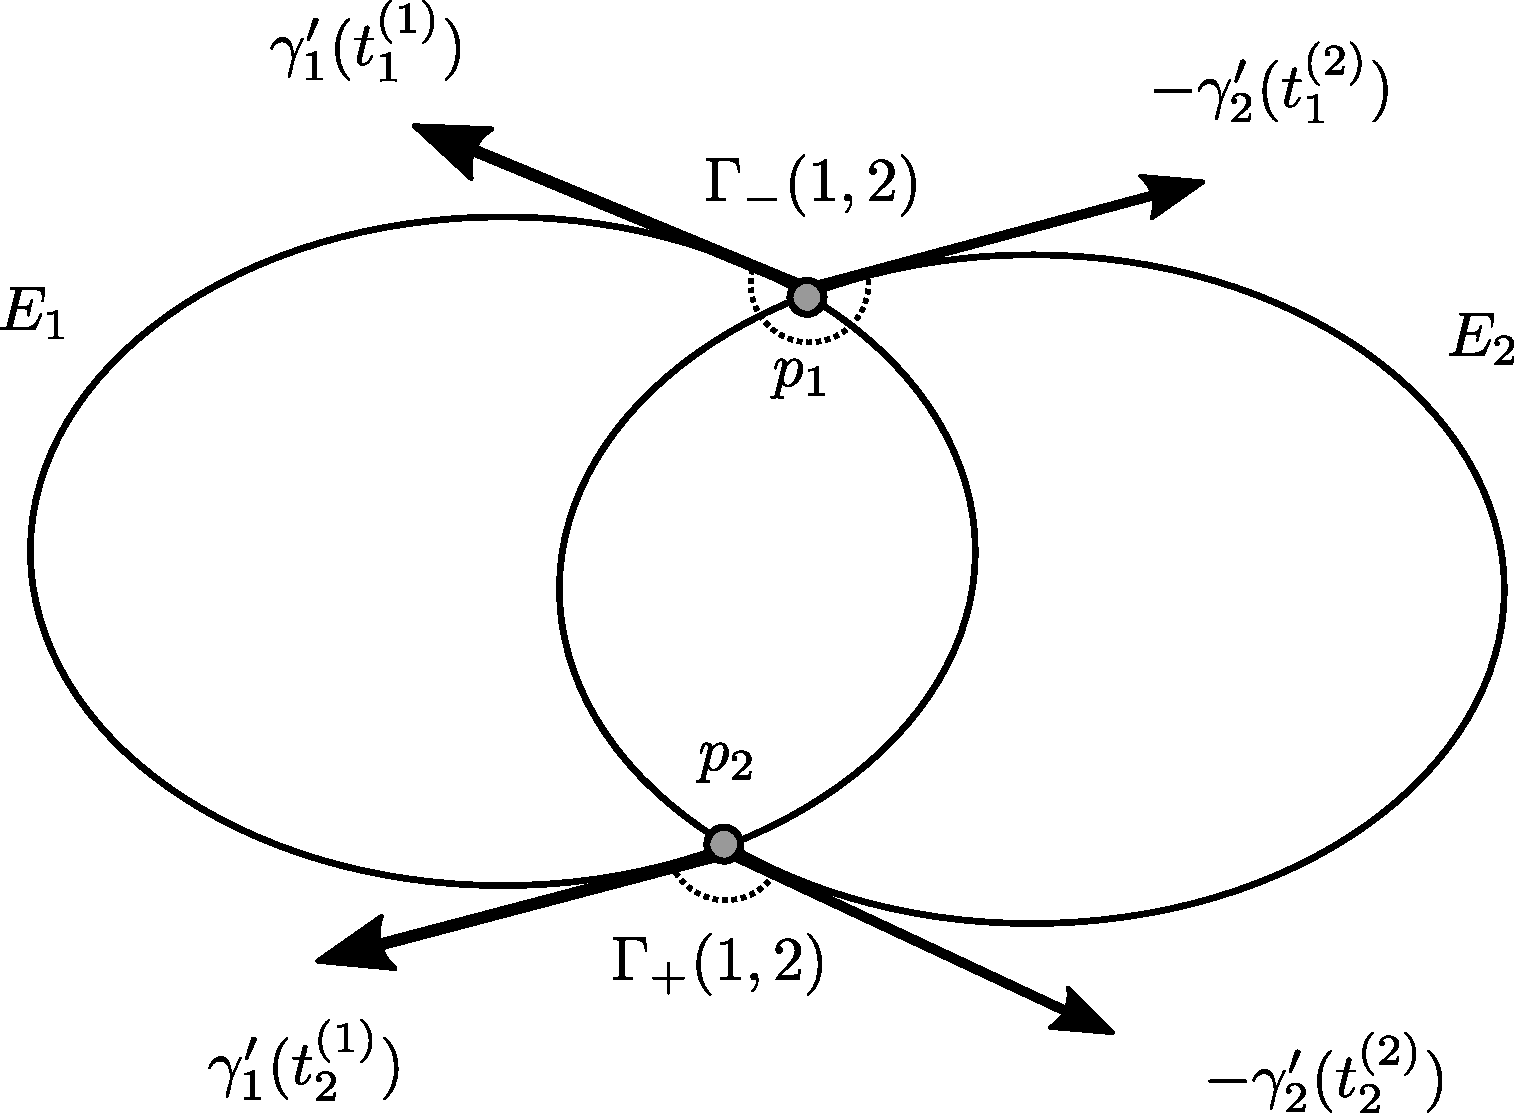
\includegraphics[scale=.38]{tex/figures/ellipse_gamma.pdf}
	\fautor
	\label{fig:ellipse_gamma}
\end{figure}

\section{An algorithm for MCE}

The same procedure defined in \autoref{algoritmo:mcd_cls} can be used to get a CLS for every ellipse in MCE. We refer to the elliptical version of that procedure as CLS-MCE (we do not define it in this chapter because it would look the same as CLS-MCD defined in \autoref{algoritmo:mcd_cls}, apart from the name, of course). 

Then, with the algorithm to construct a CLS for every ellipse in hands, an algorithm for MCE naturally comes into existence. In \autoref{algoritmo:mce}, a complete search is done backtracking every possibility in the CLS of every ellipse. This strategy is backed-up by \autoref{lema:mcd}, which says that there is an optimal solution in the CLS of each ellipse. 
Following this, counting every possibility that the algorithm goes through, we arrive at the run-time complexity of $\bigO(n^{2m})$.

It is worth mentioning that, even though we call CLS-MCE every time in the recursion, in practice, it is probably best to pre-process this step, and only call it $m$ times for the whole set of points.
Some other easy improvements can also be made in the implementation. For example, if an ellipse covers two sets of points $X$ and $Y$, with $X \subset Y$, then set $X$ can be ignored by the algorithm because of the non-negative weights constraint. Also, if two ellipses have their centers with Euclidean distance greater than their semi-major parameter, they for sure do not intersect. Depending on the input, this observation can make the algorithm not go through the whole list of ellipses every time it needs to determine the ellipses pairwise intersections.

\section{Adding facility cost}

Additionally, in \citeonline{andreta} and \citeonline{canbolat}, two other parameters are present in the definition of the problem. This extension is the result of having costs associated with every facility.
In MCE, though, the total cost, which is the sum of costs of every used facility, is constant; hence, to create a decision about which ones are utilized, a new parameter $k\in\mathbb{N}$ is given, along with a constraint on the number of used ellipses.

We refer to this version of the problem as  \sigla{MCE-$k$}{Maximum Covering by Ellipses with a $k$-constraint}. An instance of it is given by the same parameters as MCE, plus a list of costs $\Cc=\{c_1, \dots, c_m\}$, with $c_j\in\R_{\ge0}$ being the $j$-th ellipse's cost, and $k\in\mathbb{N}$, $k\le m$.

 A solution for MCE-$k$, however,  when compared to MCE's, has a bit more cluttered description. We define it as a set $I:=\{i_1, \dots, i_k\}\subset\{1, \dots, m\}$, such that $|I|=k$; and a tuple $Q:=(q_1, \dots, q_k)$, with $q_j\in\R^2$ being the center of the $j$-th ellipse in $I$. An optimal solution of MCE-$k$ is given by the optimization problem

\begin{equation*}
\max_{I, Q} w\left(\bigcup_{j=1}^k \Pp \cap E_{i_j}(q_j)\right).
\end{equation*}

Finally, \autoref{algoritmo:mce} can serve as basis for MCE-$k$'s \autoref{algoritmo:mce-k}. 
Firstly, for every subset $I \subset \{1, \dots, m\}$, such that $|I| = k$, the algorithm for MCE is invoked for the instance $(\Pp, \Ww, \{(a_j, b_j) : j \in I\})$; that is, an instance where only the ellipses in $I$ are present.
After that, by keeping track of the utilized ellipses' costs for every $I \subset \{1, \dots, m\}$, an optimal solution can be obtained.
This simple adjustment achieves a run-time complexity of $\bigO(\binom{m}{k} \times n^{2k}) = \bigO(2^mn^{2m})$. 

\begin{algoritmo}
    \caption{Algorithm for MCE}\label{algoritmo:mce}
    
    \begin{algorithmic}[1]
        \Require{A set of points $\Pp=\{p_1,\dots,p_n\}$, a list of weights $\Ww=\{w_1, \dots, w_n\}$, and a list of shape parameters $\Rr=\{(a_1, b_1), \dots, (a_m, b_m)\}$.}
        
        \Ensure{An optimal solution for MCE.}
        
        \item[]
        \Procedure{$MCE$}{$\Pp, \Ww, \Rr$}
	    \State \Return $MCE_{bt}(\Pp, \Ww, \Rr, 1)$
        \EndProcedure
        \State
        \Procedure{$MCE_{bt}$}{$Z, \Ww, \Rr, j$}
        \If{$j = m+1$}
        \State \Return $0$
        \EndIf
        
        \State $(q_j^*, \dots, q_m^*) \gets (0, \dots, 0)$

        \State $S_j \gets \textnormal{CLS-MCE}(Z, a_j, b_j)$
        \For{$q_j \in S_j$}
        \State $Cov \gets \Pp \cap E_j(q_j)$
        \State $(q_{j+1}, \dots, q_m) \gets MCE_{bt}(Z \setminus Cov, \Ww, \Rr, j+1)\}$
        
        \If{$w(\cup_{k=j}^m Z \cap E_k(q_k)) >  w(\cup_{k=j}^m Z \cap E_k(q_k^*))$}
        \State $(q_j^*, \dots, q_m^*) \gets(q_j, \dots, q_m)$
        \EndIf
        \EndFor

        \State \Return $(q_j^*, \dots, q_m^*)$
        \EndProcedure
    \end{algorithmic}
\end{algoritmo}

\begin{algoritmo}
	\caption{Algorithm for MCE-$k$}\label{algoritmo:mce-k}

	
	\begin{algorithmic}[1]
   \Require{A set of points $\Pp=\{p_1,\dots,p_n\}$, a list of weights $\Ww=\{w_1, \dots, w_n\}$, a list of shape parameters $\Rr=\{(a_1, b_1), \dots, (a_m, b_m)\}$, a list of costs $\Cc=\{c_1, \dots, c_m\}$, and $k\in \mathbb{N}$.}
	\Ensure{An optimal solution for MCE-$k$.}
	        
	\item[]
	
\Procedure{MCE-$k$}{$\Pp, \Ww, \Rr, \Cc, k$}
	\State $I^* = \{i_1^*, \dots, i_k^*\}\gets \{1, \dots, k\}$
	\State $Q^* = (q_1^*, \dots, q_k^*) \gets (0, \dots, 0)$
	
	\ForAll{$I=\{i_1, \dots, i_k\} \subset \{1, \dots, m\}$}

		\State $\Rr' \gets \{(a_j, b_j) \in \Rr: j \in I\}$
		\State $(q_1, \dots, q_k) \gets MCE(\Pp, \Ww, \Rr')$
					
		\If{$w(\bigcup_{j=1}^k \Pp \cap E_{i_j}(q_j)) - \sum_{j\in I} c_j > w(\bigcup_{j=1}^k \Pp \cap E_{i_j^*}(q_j^*)) - \sum_{j\in I^*}c_{j}$}
			\State $Q^* \gets (q_1, \dots, q_k)$
			\State $I^* \gets I$
		\EndIf
	\EndFor
	
	\State \Return $I^*, Q^*$
\EndProcedure
	\end{algorithmic}
\end{algoritmo}